\chapter{Estabilidad de los Amplificadores Realimentados}\label{estabilidad}

{\hspace{10pt}} La estabilidad de un amplificador está relacionada en forma directa con la ubicación de los polos de su función transferencia. Un amplificador es estable si todos los polos de su función transferencia, definida en el plano s, poseen parte real negativa. En forma cualitativa se muestra en la figura \ref{estab1} la respuesta transitoria al impulso de un amplificador en función de la posición de sus polos. En las figuras \ref{estab1}a) y b) el amplificador es estable, en la c) presenta oscilaciones sostenidas y en las d) y e) su comportamiento
es inestable.

En los análisis que se realizarán se parte de la suposición que el amplificador sin realimentar (a(s)) tiene todos sus polos en el semiplano izquierdo, es decir es estable. Al realimentarlo los polos de la transferencia total (A(s)) se mueven, pudiendo hacerlo hacia zonas de inestabilidad, es por lo tanto importante el estudio de estos movimientos para determinar la estabilidad del amplificador.

El esquema básico de un amplificador realimentado es el mostrado en la figura \ref{real1}, ya presentado en el capítulo anterior. Considerando ahora que las transferencias están definidas en el plano s, se tiene que:

\begin{equation}\label{ecuestab1}
	A(s)=\frac{\displaystyle a(s)}{\displaystyle 1+T(s) } \quad \quad \text{con }  T(s)=a(s)\textsf{f}(s)
\end{equation}




Los polos de A(s) del sistema realimentado son las raíces de la ecuación característica, $1 + T (s) = 0$. Los métodos que se utilizan para analizar la estabilidad de los amplificadores realimentados, se basan en el concepto de estudiar el comportamiento de las raíces de la mencionada ecuación característica.

\begin{figure}[h]
	\centering
	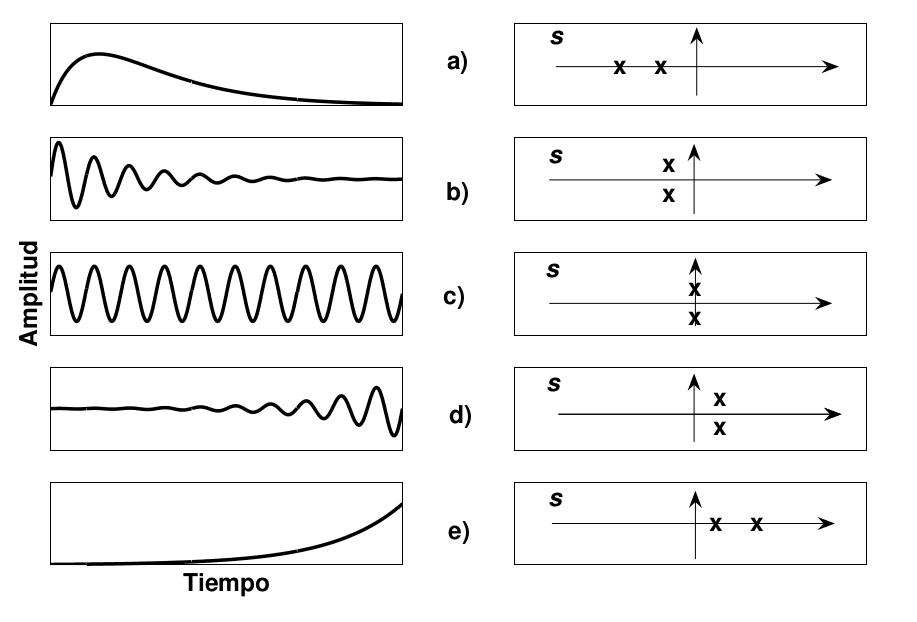
\includegraphics[width=0.6\linewidth]{figuras/estab1.png}
	\caption{Relación entre la ubicación de los polos y respuesta transitoria.}
	\label{estab1}
\end{figure}


\section{Transferencias teóricas}

\hspace{10pt} Se pueden utilizar las herramientas del LTSpice para analizar y diseñar transferencias realimentadas teóricas y estudiar su comportamiento con respecto a la estabilidad.

Por ejemplo si se tiene un amplificador sin realimentar pasa bajos de un sólo polo cuya transferencia es:

  \begin{equation}
  	a(s)=\frac{\displaystyle a_o}{\displaystyle 1+\frac{s}{2\pi f_p} }
  \end{equation}
  con  ganancia de continua $a_o=100$ y un polo en $f_p=1KHz$ y se lo realimenta con una transferencia de realimentación $f=0.1$ independiente de la frecuencia, se obtiene reemplazando estos valores en la ecuación \ref{ecuestab1}:
   \begin{equation}
  	A(s)=\frac{\displaystyle A_o}{\displaystyle 1+\frac{s}{2\pi f_{pf}} }
  \end{equation}
  con $T_o=a_of=10$ el valor de la ganancia de lazo en continua,  $A_o=\frac{\displaystyle a_o}{\displaystyle 1+T_o}=9.0909$ la ganancia realimentada en continua y $f_{pf}=(1+T_o)f_p=11Khz$ la frecuencia del polo realimentado. 
  
  Este comportamiento es muy conocido en la teoría de realimentación y puede ser estudiado utilizando LTSpice. En la figura \ref{estab2} se muestra la implementación del sistema teórico, la fuente controlada  $E_1$ representa la transferencia $a(s)$ sin realimentar, para que dependa de $s$ se debe definir el parámetro \textit{SpiceModel=laplace} y en \textit{value} se debe definir la transferencia correspondiente en función de s, ver la pantalla desplegada a la izquierda de la figura mencionada. La fuente controldada $E_2$ representa a la realimentación f, las resistencias $R_1$ y $R_2$ se colocan para dar conexión al circuito pero no influyen en el resultado. En la figura \ref{estab3} se muestran los diagramas de Bode de amplitud y fase de  la simulación de la transferencia $A(jf)$ en rojo, que es la ganancia entre la salida y la entrada y la transferencia sin realimentar $a(jf)$ en azul que es la ganancia entra la salida y la entrada de la fuente controlada $E_1$. Los resultados coinciden con los calculados anteriormente.
  
  
\begin{figure}
	\centering
	
\includegraphics[width=1.0\linewidth]{figuras/estab2.png}
	\caption{Implementación circuital de un circuito realimentado teórico.}
	\label{estab2}
\end{figure}

\begin{figure}
	\centering
	
\includegraphics[width=0.8\linewidth]{figuras/estab3.png}
	\caption{Diagramas de Bode del circuito teórico de un polo.}
	\label{estab3}
\end{figure}

Se puede extender este análisis utilizando el circuito de la figura \ref{estab2} si se cambia las transferencias de la fuentes controlada $E_1$ y $E_2$. Por ejemplo si mantenemos la misma realimentación $f=0.1$ y agregamos un polo más de $2KHz$ a la transferencia:

\begin{equation}\label{ecuestab2}
	a(s)=\frac{\displaystyle a_o}{\displaystyle (1+\frac{s}{2\pi 1000})(1+\frac{s}{2\pi 2000}) }
\end{equation}

En la figura \ref{estab4} se muestran los diagramas de Bode de amplitud y fase de las transferncias $A(jf)$ y $a(jf)$, en rojo y en azul respectivamente. Evidenciando $A(jf)$ el conocido comportamiento de un sistema de segundo orden con polos complejos conjugados.

\begin{figure}
	\centering
	
\includegraphics[width=0.8\linewidth]{figuras/estab4.png}
	\caption{Diagramas de Bode del circuito de segundo orden.}
	\label{estab4}
\end{figure}
 
 Se puede también analizar la respuesta temporal utilizando la fuente $V_1$ del circuito de la figura \ref{estab2} como una fuente pulsada tipo \textit{PULSE(0 .5 0 1u 1u 1m 2m)} y ejecutar la directiva \textit{.tran 0 4m 0 1u}. En la figura \ref{estab5} se muestra en la parte superior la entrada y en la inferior la salida, mostrando el comportamiento oscilatorio amortiguado del sistema.
 
 \begin{figure}
 	\centering
 	
\includegraphics[width=0.8\linewidth]{figuras/estab5.png}
 	\caption{Respuesta temporal del circuito de segundo orden.}
 	\label{estab5}
 \end{figure}
 
 \section{Criterio de estabilidad de Bode}
 
 \hspace{10pt} Se puede utilizar el LTSpice para determinar la estabilidad de un amplificador mediante el criterio de Bode \cite{gray95}.
 
 Si se utiliza la transferencia sin realimentar de segundo orden de la ecuación \ref{ecuestab2} con una red de realimentación $\textsf{f}=0.5$ se puede analizar la estabilidad utilizando el circuito de la figura \ref{estab6}, en la parte superior se implementa la ganancia sin realimentar $a(s)$ a través de la fuente de tensión controlada $E_1$ y la realimentación $\textsf{f}=0.5$ por medio de la fuente $E_2$, visualizando los nodos $a$ y $t$ se obtienen los diagramas de Bode de $a(jf)$ y $T(jf)$ respectivamente. En el mismo circuito, en la parte inferior se implementa el sistema realimentado con las fuentes controladas $E_3$ y $E_4$, en el nodo $o$ se obtiene la transferencia realimentada $A(jf)$.  En la figura \ref{estab7} se muestran las transferencias de $a(jf)$ en verde, la de $A(jf)$ en rojo y la de la ganancia de lazo $T(jf)$ en azul, utilizando el criterio de Bode se encuentra que el sistema es estable pero con un margen de fase exiguo de $\approx 17.3^{\circ}$, como consecuencia de ello se observa un elevado sobrepico en la transferencia $|A(jf)|$ a las frecuencias donde el $|T|\approx1$.
 

 
  \begin{figure}
 	\centering
 	
\includegraphics[width=1.0\linewidth]{figuras/estab6.png}
 	\caption{Utilización del criterio de estabilidad de Bode en una transferencia realimentada teórica. }
 	\label{estab6}
 \end{figure}
  \begin{figure}
 	\centering
 	
\includegraphics[width=0.8\linewidth]{figuras/estab7.png}
 	\caption{Transferencias teóricas y medición del margen de fase.}
 	\label{estab7}
 \end{figure}
 
 En los circuitos prácticos no siempre se puede identificar fehacientemente las funciones transferencias involucradas, por lo que el método teórico propuesto anteriormente puede no ser aplicable o aplicable con un apreciable margen de error al estimar las transferencias. En estos casos se puede utilizar el método de obtención de la ganancia de lazo desarrollado en el capítulo anterior, es decir se analizará la transferencia de la ganancia de lazo $T(jf)$ y se le aplicará el criterio de Bode. 
 
 En la figura \ref{estab8} se muestra un circuito realimentado con dos fuentes de alterna $V_4$ y $V_3$, la primera es la entrada al circuito y la segunda es la fuente de prueba insertada en un nodo que presenta alta impedancia para obtener la ganancia de lazo. Si se quiere hallar la ganancia de tensión entre la entrada $V_4$ y la salida $V_o$ se debe ajustar a 1V a la fuente $V_4$ y a 0V a la fuente $V_3$, por el contrario si se quiere hallar la ganancia de lazo hay que ajustar las fuentes $V_4$ a 0V y la $V_3$ a 1V. El parámetro $k$ definido por la directiva Spice \textit{.param k=0} significa que el capacitor $C_2=k*5pF=0$. Las figuras \ref{estab9} y \ref{estab10} representan la ganancia de lazo y la ganancia de tensión realimentada respectivamente. El criterio de Bode se aplica en la ganancia de lazo y se muestra en la figura correspondiente, observando que el margen de fase es positivo, y por lo tanto estable, pero de valor exiguo ($\approx 8.7^{\circ})$ lo que deviene en el elevado sobrepico en la ganancia de tensión mostrado en la figura \ref{estab10}, en dicha figura se observa también que la frecuencia a la que ocurre el sobrepico es de $3.01MHz$ y su valor es de $37.76dB$ que es $\approx17dB$ por encima del valor observado a frecuencias bajas.
 
 \begin{figure}
 	\centering
 	
\includegraphics[width=1.0\linewidth]{figuras/estab8.png}
 	\caption{Obtensión de las ganancias realimentadas y de lazo en un circuito práctico. }
 	\label{estab8}
 	 \end{figure}
 	 
 	 
 	 \begin{figure}
 	 	\centering
 	 	
\includegraphics[width=0.7\linewidth]{figuras/estab9.png}
 	 	\caption{Ganancia de lazo del circuito de la fig \ref{estab8} con $C_2=0$. Margen de fase.}
 	 	\label{estab9}
 	 \end{figure}
 	 
 	 \begin{figure}
 	 	\centering
 	 	
\includegraphics[width=0.7\linewidth]{figuras/estab10.png}
 	 	\caption{Ganancia de tensión del circuito de la fig \ref{estab8} con $C_2=0$.}
 	 	\label{estab10}
 	 \end{figure}
 	 
 	 \section{Compensación de la ganancia de lazo}
 	 
 	 \hspace{10pt} Si un amplificador es inestable o tiene un margen de fase pequeño, como es el caso del circuito de la figura \ref{estab8}, se deben realizar las acciones necesarias para aumentar el margen de fase para que el amplificador deje de ser inestable y tenga el margen de fase suficiente para que su respuesta sea satisfactoria, estas acciones se denominan compensación de la realimentación.
 	 
 	 En general compensar un amplificador realimentado es actuar sobre la ganancia de lazo $T(s)$ de modo de obtener un margen de fase determinado, sin modificar la ganancia realimentada a frecuencias bajas o medias $A_o$. Para que las respuestas en frecuencia y temporal sean adecuadas se considera, desde el punto de vista práctico, que los amplificadores deberán tener un margen de fase de al menos  $45^{\circ}$.
 	 
 	 Como se mencionó antes, para compensar un amplificador se debe actuar sobre $T(s)$. La mayoría de los métodos de compensación actúan directamente sobre la ganancia sin realimentar $a(s)$, suponiendo realimentación unitaria ($\textsf{f}= 1$), compensándolo para tener un margen de fase de $\approx 45^{\circ}$, $\textsf{f}= 1$ es el peor caso desde el punto de vista de la estabilidad por lo que la compensación estará asegurada para cualquier otro caso. Esta estrategia es la que se sigue en general con los amplificadores operacionales, utilizando los métodos de compensación por polo dominante y compensación por corrimiento del primer polo, ambos métodos actúan sobre la ganancia $a(s)$ y por lo tanto en $T(s)$ \cite{gray95}.
 	 
 	 Otro método utilizado frecuentemente es el denominado compen\-sa\-ción por adelanto de fase o compen\-sa\-ción mediante el agregado de un cero en la realimentación \cite{gray95}. El agregado de un cero a la ganancia de lazo $T(jf)$ a la frecuencia $f_{0dB}$, en que $|T(jf_{0dB})| = 1$; produce una mejora de $45^{\circ}$ en el margen de fase en el sistema compensado. Esto se debe a que el cero agregado aporta $+45^{\circ}$ a la fase total a dicha frecuencia, sin modificar apreciablemente el pasaje por $0dB$ de $|T(jf)|$. En general en un amplificador realimentado, agregar un cero en $T(s)$ implica la ubicación de algún componente reactivo; esto agrega además algún polo adicional a la transferencia. Si dicho polo adicional se encuentra a una frecuencia mucho mayor que la frecuencia del cero agregado, el cero producirá el efecto ya explicado. Lo importante de este método es que el cero agregado a $T(s)$ se logra, en los casos prácticos, haciéndolo sobre la realimentación $\textsf{f}(s)$ y no sobre la ganancia $a(s)$.
 	 
 	 
 	 	 \begin{figure}[t]
 	 	\centering
 	 	
\includegraphics[width=0.7\linewidth]{figuras/estab11.png}
 	 	\caption{Ganancia de tensión para $C_2=0$, $C_2=3pF$ y $C_2=5pF$}
 	 	\label{estab11}
 	 \end{figure}
 	 
 	 
 	  Para dar un ejemplo se utiliza el circuito de la figura \ref{estab8}, en el punto anterior se analizó el caso en el que el capacitor $C_2=0$ y se vio que el margen de fase era pequeño y que en la respuesta en frecuencia de $|A(jf)|$ se producía un pronunciado sobrepico. Si se considera ahora una capacidad $C_2 \neq 0$ en paralelo con $R_3$ se puede observar en dicha figura que la red de realimentación estará ahora compuesta por $R_3$, $R_2$ y $C_2$. Utilizando esa red se pueden obtener sus parámetros $\textit{h}$ y particularmente:
 	 
 	 
 	 \medskip
 
 	 
 	 \begin{equation}\label{ecuestab3}
 	 	\textsf{f}(s)=h_{12}=\frac{\displaystyle R_2}{\displaystyle R_2+R_3}\frac{\displaystyle (1+sC_2R_3)}{\displaystyle (1+sC_2R_3||R_2)}
 	 \end{equation}
 	 
 	 
 	 \medskip

 
 	 
 	 En esta ecuación se ve que a la red $\textsf{f}$ tiene ahora un cero en $f_o=\frac{1}{2\pi C_2R_3}$ y un polo en $f_p=\frac{1}{2\pi C_2R_3||R_2}$, estas singularidades se agregarán a la transferencia de $T(s)$. En principio se puede suponer que los efectos de carga adicionales agregados por $C_2$ a la ganancia $a(s)$ no son apreciables y que el polo que se agrega está a una frecuencia superior que no afecta en las inmediaciones del pasaje de $|T(jf)|$ por $0dB$. Si no se cumplieran estas suposiciones deberían tenerse en cuenta sus efectos.
 	 
 	 El cero debe ser agregado a la frecuencia en que $|T(jf)|=1$ ($0dB$), en el caso de la figura \ref{estab8} con $C_2=0$ esa frecuencia es de $\approx 3MHz$ que coincide aproximadamente con la frecuencia en la que se produce el sobrepico en la ganancia $|A(jf)|$ \cite{gray95}. En este caso entonces el capacitor que debe ser agregado es:
 	 
 	 
 	 \medskip
 
 	 
 	 \begin{equation}\label{ecuestab4}
 	 C_2=\frac{\displaystyle 1}{\displaystyle 2\pi R_3f_o}=\frac{\displaystyle 1}{\displaystyle 2\pi 10K3MHz}=5.3pF
 	 \end{equation}


\medskip

 	 
 	 
 	 En la figura \ref{estab8} está puesta como comentario la directiva Spice \textit{.step param k list 0 0.6 1}, habilitando esta directiva se obtiene un barrido del parámetro k en tres valores 0, 0.6 y 1. Lo que se logra con esto es realizar el cálculo de \textit{.ac dec 1000 1 10meg} tres veces para $C_2$ igual a $0$, $3pF$ y $5pF$ respectivamente. En la figura \ref{estab11} se muestra la ganancia realimentada para cada caso del parámetro k, a medida que aumenta el valor de $C_2$ disminuye el sobrepico y por lo tanto aumenta el margen de fase. Para $k=1$ ($C_2=5pf$), prácticamente se elimina el sobrepico. 
 	 
 	 	    
 	   
 	   
 	   